\chapter{Tests}
\label{chap:Tests}

Aus zeitlichen Gründen musste die Testphase gekürzt werden. Es konnten somit keine Testversuche auf dem Packpot durchgeführt werden. Nachfolgend wurden Funktionstests durchgeführt, damit eruiert werden kann, welche Funktionen erreicht wurden.

\section{Testspezifikationen}
\label{sec:Testprotokolle}
Nachfolgende Tabelle, \ref{fig:funktest} gibt einen Überblick, welche Teilfunktion getestet werden. Dabei wird kurz ein Beschrieb dazu geliefert und welche Parameter bzw. Spezifikationen ausgewertet werden. 

\begin{table}[H]
	\centering
	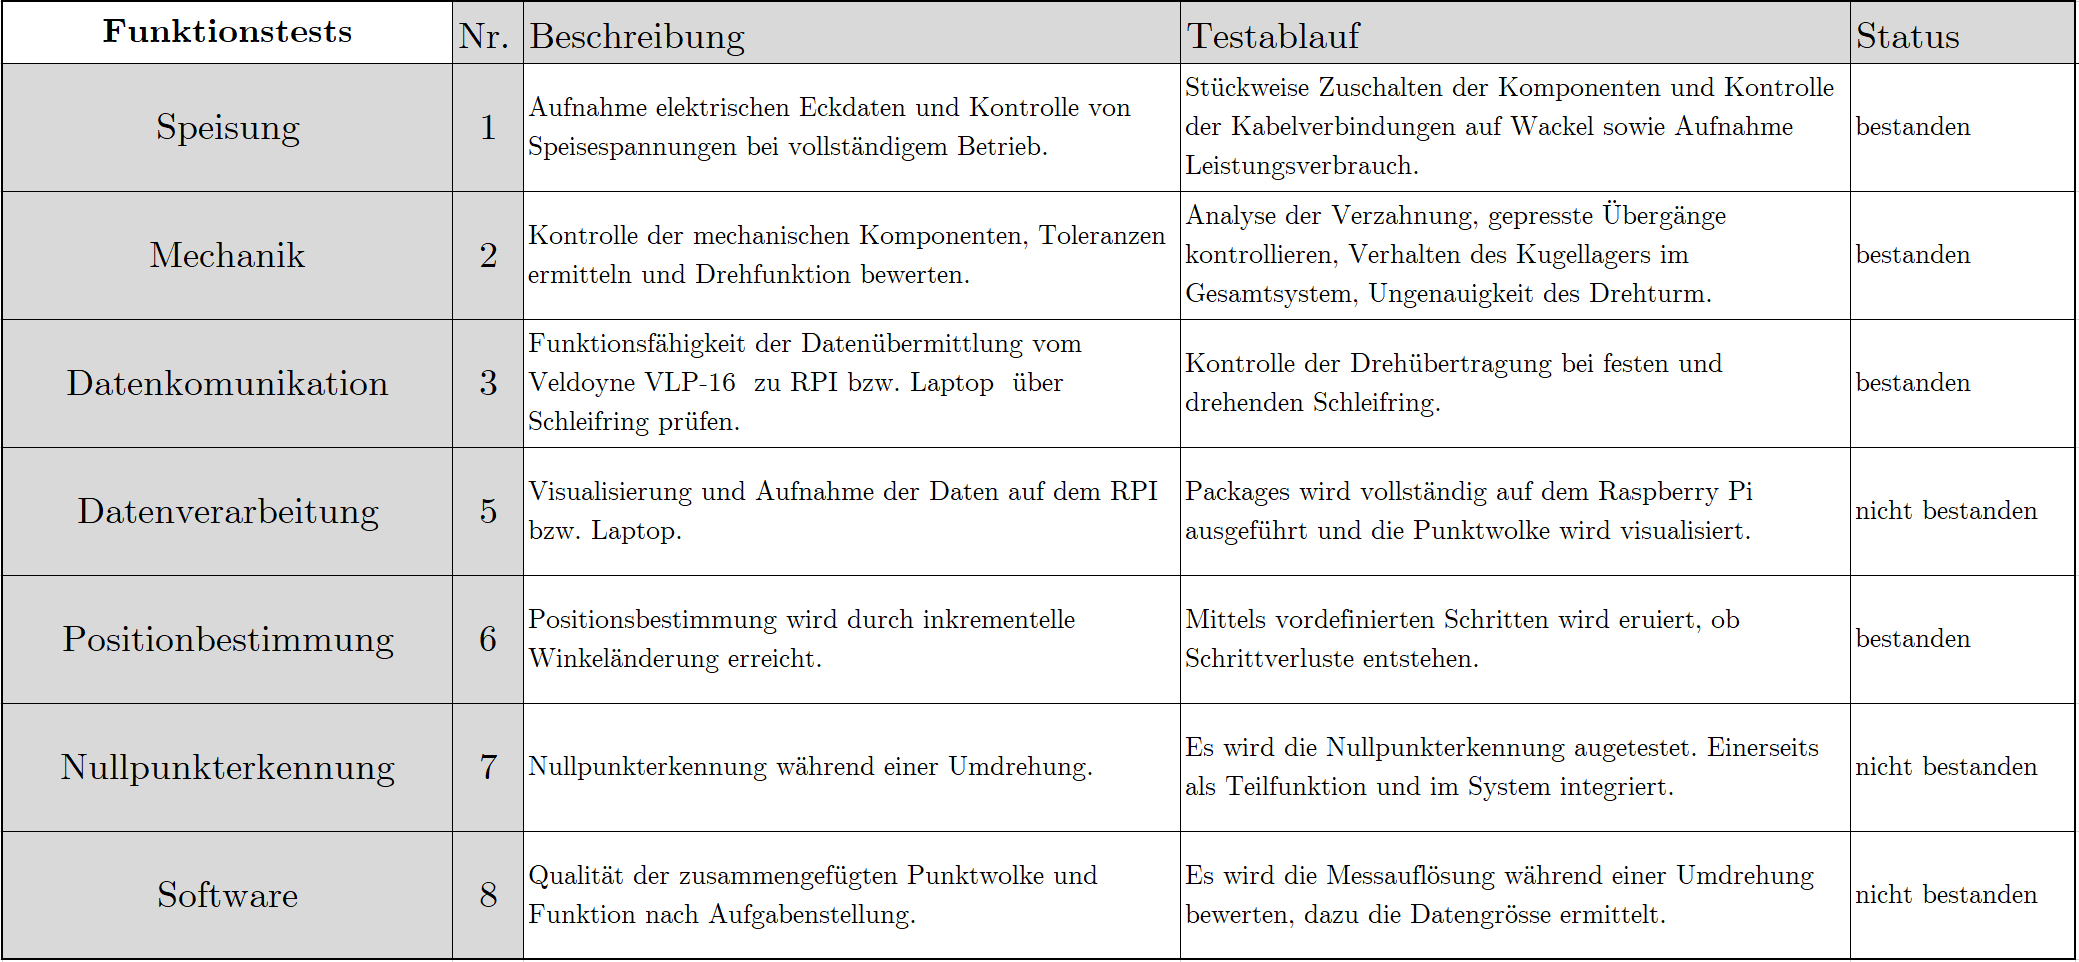
\includegraphics[,width=1\textwidth]{resources/Testtabelle.PNG}
	\caption[Funktionstest im Überblick]{Funktionstests im Überblick}
	\label{fig:funktest}
\end{table} 

\section {Testergebnisse}
\label{sec:Testergebnisse}
Die definierten Testergebnisse werden 

\subsection {Speisung}
\label{subsec:Speisung}
Mittels einem ROHDE \& SCHWARZ NGSM32 wurde eine exakte 12 Volt Speisung zugeführt. Alle Komponenten konnten problemlos zugeschaltet werden. Wackelkontakte wurden keine festgestllt. Die Leistungsaufnahme der gesamten Modul variiert zwischen 9-15 Watt. Dies ist abhängig von der auszuführenden Funktion. Da keine Mängel festgestellt wurden, gilt dieser Funktionstest als erfüllt.
\subsection {Mechanik}
\label{subsec:Mechanik}
Die Mechanik wurde auf Mängel geprüft. Die zwei Zahnräder verlaufen sehr exakt ineinander und verkanten sich nicht. die gepressten Teile sitzen fest und verursachen keine Toleranzen. Einzig der Kugellageradapter ist nicht optimal gepresst. Dies verursacht, dass der drehende Hohlzylinder den Abstand zum QRE 1113 um einen Millimeter variiert. Da die Mechanik ansonsten einwandfrei funktioniert gilt dieser Funktionstest als bestanden.

\subsection {Datenkommunikation}
\label{subsec:Datenkimmuikation}
Die Datenkommunikation ist in allen Fällen gewährleistet. Es kann zwischen dem Velodyne VLP-16, dem Raspberry Pi 3 und dem Laptop problemlos kommuniziert werden. Es wurden mehrere Datensätze auf vollständige Messages geprüft. Dabei konnten keine fehlenden Messages festgestellt werden. Die Datensätze wurden mit rotierendem Turm, sowie mit den Drehgeschwindigkeiten von 5$^\circ$/s, 20$^\circ$/s und 120$^\circ$/s fehlerlos übermittelt.  

\subsection {Datenverarbeitung}
\label{subsec:Datenverarbeitung}
Die Datenverarbeitung des Datenstreams wurde auf dem Raspberry Pi, wie auch auf dem Laptop geprüft. Beim Raspberry Pi 3 besteht das Problem, dass die Visualisierung mit Rviz mangelhaft funktioniert. Aufgrund der Datenrate von 8 Mbit/s steigt die Grösse der Punktwolke schnell an. Das Raspberry Pi stösst für die Visualisierung dieser Punktwolke an die Grenzen. Auf dem Laptop konnten die Punktwolke in Echtzeit visualisiert werden, da dieser bedeutend höhere Rechenleistungen bietet. 

\subsection {Positionsbestimmung}
\label{subsec:Positionsbestimmung}

\subsection {Nullpunkterkennung}
\label{subsec:testSNullpunkterkennung}
Die Nullpunkterkennung besitzt Mängel. Der Nullpunkt wurde bei den Mündungsgeschwindigkeiten von 5$^\circ$/s, 20$^\circ$ und 120 $^\circ$ nicht vollständig erkennt. Dabei wurden aus den Datensätzen 

\subsection {Software}
\label{subsec:testSoftware}

\section{Zwischenfazit}
\label{sec:Fazit}

Die Test geben Überblick, welche Funktionsbereiche überarbeitet werden müssen bzw. bei welchen noch zufriedenstellende Ergebnisse geliefert werden.
Dieser Testaufbau zeigt auf, dass für die Ansteuerung der Aktoren und Sensoren ein Raspberry Pi gute Dienste leistet. Für die Visualisierung benötigt es jedoch leistungsfähigere Rechenmaschinen.  